\documentclass[a4paper, 12pt, oneside]{article}

\usepackage[utf8]{inputenc}
\usepackage[T1]{fontenc}
\usepackage{lmodern} % Enlève plein de warnings :D et permet le tt gras
\usepackage[french]{babel}

% \usepackage[usenames,dvipsnames,svgnames,table]{xcolor}

\usepackage{amsmath}
\usepackage{amssymb}
% \usepackage{mathrsfs}

\usepackage{hyperref}
\usepackage{scrextend}

\usepackage{graphicx}

\usepackage{color}
\usepackage{listings}
\definecolor{listinggray}{gray}{0.9}
\definecolor{lbcolor}{rgb}{0.95,0.95,0.95}
\lstset{
	backgroundcolor=\color{lbcolor},
	tabsize=4,
	rulecolor=,
	language=Java,
	basicstyle=\scriptsize\ttfamily,
	upquote=false,
	aboveskip={.5\baselineskip},
	columns=fixed,
	showstringspaces=false,
	extendedchars=true,
	showspaces=false,
	breaklines=true,
	prebreak = \raisebox{0ex}[0ex][0ex]{\ensuremath{\hookleftarrow}},
	frame=single,
	showtabs=false,
	identifierstyle=\ttfamily,
	keywordstyle=\bfseries\color[rgb]{0,0,1},
	commentstyle=\color[rgb]{0.133,0.545,0.133},
	stringstyle=\color[rgb]{0.627,0.126,0.941},
}

% ---------------
% Commmandes
% ---------------

% Argument obligatoire : nom du type agrégé
\newenvironment{typeag}[1][]{\noindent \textbf{type} \texttt{#1} \{\begin{addmargin}[2em]{0em}}{\end{addmargin}\}}
% Arguments obligatoires : Nom — Type — Description
\newcommand{\variable}[3]{\noindent \texttt{#1} : \textit{#2} --- #3}

%Déclaration de variables
\newcommand{\var}[1]{\texttt{#1}}

% Algorithme informel % Ou \scriptsize
\newenvironment{algoinfo}{\begin{itemize}\small}{\end{itemize}}

% \renewcommand\arraystretch{1.2}

\newcommand{\oeuvre}[1]{\textit{#1}}

\newcommand{\lien}[2]{\noindent #1 :\\{\small\url{#2}}}

% ---------------
% Main
% ---------------
\title{Manuel du programme Démineur}
\author{Mohamed \bsc{Lakhal}\\Alexis \bsc{Cabodi}}
\date{Révision du\\\today}

\begin{document}
\maketitle
\newpage
\tableofcontents
\newpage

\section{Mode d'emploi}
Le but du jeu est de découvrir toutes les cases non minées en évitant de cliquer sur une case minée. Le joueur a la possibilité de poser un drapeau sur une case qu'il soupçonne contenir une mine. Attention, le drapeau peut aussi être posé sur une case quelconque. Il faudra donc les placer avec autant de réflexion qu'en découvrant une case.
\bigskip

Après le lancement de l'application, le joueur saisit divers paramètres afin d'initialiser sa partie : nombre de lignes (entre 3 et 50 inclus), de colonnes (entre 3 et 80 inclus) et de mines (au moins une et moins que le nombre de cases).
À l'aide du clic gauche de la souris, le joueur peut découvrir une case. Avec le clic droit, il pose un drapeau sur la case. Ce drapeau assure le joueur qu'il ne pourra pas découvrir une mine par accident puisqu'il faudra retirer le drapeau à l'aide d'un autre clic droit pour pouvoir découvrir la case.
\bigskip

En cours de jeu, le joueur peut voir à tout moment le temps écoulé depuis son premier placement de drapeau ou découvrement de case. Le chronomètre en haut à droite s'arrêtera en même temps que la partie, ce qui permet de voir le temps de jeu total à la fin.
\bigskip

Si le joueur découvre une case minée, il perd et donc la partie s'arrête.
Le joueur gagne et la partie se termine si l'une des deux conditions suivantes est satisfaite :
\begin{itemize}
	\item L'ensemble des cases non minées et uniquement ces cases sont découvertes. Les drapeaux placés n'influent pas ;
	\item L'ensemble des cases minées et uniquement ces cases contiennent un drapeau. Les cases découvertes n'influent pas.
\end{itemize}
\smallskip

\begin{figure}[htp]
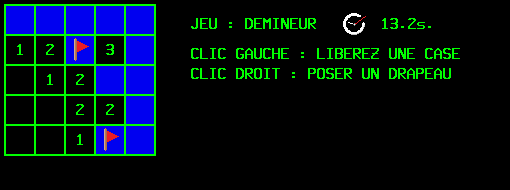
\includegraphics[width=\columnwidth]{Exemple.png}
\caption{Partie s'aidant des drapeaux}
\label{fig:picApercu}
\end{figure}

\newpage
\section{Développement}
Cette section va traiter des divers aspects liés au développement de l'application.
\subsection{Résolution des problèmes}

\subsubsection{Types agrégés}
Le premier problème était d'abord de représenter les informations du jeu de manière compréhensible par l'ordinateur. Nous avons finalement décidé de structurer ces données en deux types agrégés. Ces types, accompagnés de quelques tableaux bidimensionnels pour les images, suffisent à décrire ces informations. D'abord une case du jeu, qui sera ajoutée autant de fois que nécessaire dans la grille faisant partie de l'autre type agrégé. À noter que pour simplifier l'écriture du programme, la grille est une variable indépendante de \var{Demineur} dans le code source.

\smallskip
\begin{typeag}[Case]
	\variable{visible}{booléen}{indique si la case est découverte} \\
	\variable{drapeau}{booléen}{indique si la case a un drapeau} \\
	\variable{contenu}{entier}{vaut $-1$ si la case contient une mine sinon indique le nombre de mines adjacentes}
\end{typeag}

\begin{typeag}[Demineur]
	\variable{nl}{entier}{nombre de lignes} \\
	\variable{nc}{entier}{nombre de colonnes} \\
	\variable{nm}{entier}{nombre de mines} \\
	\variable{tempsDebut}{réel}{temps de référence en millisecondes enregistré lors de la première action} \\
	\variable{grille}{Tableau [nc][nl] de Case}{représente la grille de jeu} \\
	\variable{tailleX}{entier}{position de référence en pixels pour les messages à droite (largeur de la grille)} \\
	\variable{tailleY}{entier}{taille de référence en pixels pour la hauteur de la fenêtre}
\end{typeag}\smallskip

\subsubsection{Divers problèmes}
Passons maintenant en revue tous les sous-problèmes qui composent un jeu tel que le Démineur.

\begin{figure}[hpt]
	\center
	\caption{\label{fig:constantes} Constantes globales en début de programme}
\begin{lstlisting}
// Constantes pour la lisibilite et la comprehension
final static int MINE = -1; // Valeur arbitraire pour indiquer qu'une case contient une mine
final static int TAILLE_CASE = 29; // EcranGraphique rajoutera un pixel de bordure a droite et en bas
// Statuts de la grille
final static int JOUABLE = 0;
final static int GAGNEE = 1;
final static int PERDUE = 2;
\end{lstlisting}
\end{figure}

\paragraph{Initialisation du jeu} Tout d'abord, nous avons dû initialiser notre jeu, c'est à dire l'interface que rencontrera l'utilisateur. Ainsi, notre premier problème a été la création d'une fenêtre de jeu adaptée à différentes tailles de grille. Pour cela nous avons utilisé la classe \var{EcranGraphique} qui nous a été donnée pour ce projet. Plus particulièrement, on appelle sa fonction \var{EcranGraphique.init}. On se sert pour cela de notre type agrégé \var{Demineur}. Ainsi, notre fenêtre de jeu s'adapte en fonction du nombre de lignes et de colonnes choisi par l'utilisateur tout en laissant de la place pour les instruction et le message de fin de partie.

\begin{figure}[hpt]
	\center
	\caption{\label{fig:fnInitialiserFenetre} Fonction \var{initialiserFenetre}}
\begin{lstlisting}
static void initialiserFenetre(Demineur dem)
{
	dem.tailleX = 10 + dem.nc * (TAILLE_CASE+1);
	dem.tailleY = 10 + dem.nl * (TAILLE_CASE+1);
	EcranGraphique.init(50, 50, dem.tailleX+390, dem.tailleY+110, dem.tailleX + 350, dem.tailleY + 30, "Demineur");
	EcranGraphique.setClearColor(0, 0, 0);
}
\end{lstlisting}
\end{figure} 

\paragraph{Initialisation de la grille} Concernant ce problème, nous devions initialiser notre grille en prenant en compte le nombre de cases et de mines. Il fallait alors tirer aléatoirement les coordonnées de \emph{différentes} cases minées et compter le nombre de mines adjacentes aux cases de coordonnées $(x,y) \iff (colonne, ligne)$. Le type agrégé \var{Demineur} a donc été nécessaire. La fonction est assez longue car il nous a fallu prendre en compte tous les cas afin de compter les mines adjacentes dans toutes les directions sauf celles qui nous font sortir de la grille.

\paragraph{Affichage} L'affichage de l'état du jeu est une partie très importante dans un jeu. En utilisant des fonctions simples, on peut construire une interface pratique pour l'utilisateur. Avec \var{EcranGraphique} et contrairement à une sortie console simple, on peut dessiner les formes dans n'importe quel ordre, tant qu'on indique la nouvelle couleur. Cela permet de regrouper dans des boucles le traçage de formes répétitives telles que les cases. Ces cases sont ici des bordures de rectangles placées côte à côte puis remplies soit avec une image de drapeau ou de mine, soit le cache bleu d'une case masquée, soit le nombre de mines adjacentes. Rien n'est écrit si ce nombre est nul. Le texte à côté est affiché assez simplement avec \var{EcranGraphique.drawString}.

Si aucune action n'est effectuée, la boucle de jeu continue et l'image est rafraîchie. On voit ainsi le chronomètre s'actualiser tout le temps.

\begin{figure}[hpt]
	\center
	\caption{\label{fig:fnAfficher} Fonction \var{afficher}}
\begin{lstlisting}
static void afficher(Demineur dem, Case [][] grille, int[][] imageFlag, int[][] imageMine, int[][] imageClk)
{
  EcranGraphique.clear();
  EcranGraphique.setColor(0, 255, 0);
  EcranGraphique.drawRect(4, 4, 1+(TAILLE_CASE+1)*dem.nc, 1+(TAILLE_CASE+1)*dem.nl);
  for(int l = 0; l < dem.nl; l++) {
    for(int c = 0; c < dem.nc; c++) {
      EcranGraphique.setColor(0, 255, 0);
      EcranGraphique.drawRect(5+(TAILLE_CASE+1)*c, 5+(TAILLE_CASE+1)*l, TAILLE_CASE, TAILLE_CASE);
      if (grille[c][l].visible) {
        if (grille[c][l].contenu == MINE) {
          EcranGraphique.drawImage(6+(TAILLE_CASE+1)*c, 6+(TAILLE_CASE+1)*l, imageMine);
        } else if (grille[c][l].contenu > 0) {
          EcranGraphique.drawString(15+(TAILLE_CASE+1)*c, 26+(TAILLE_CASE+1)*l, EcranGraphique.COLABA8x13, ""+grille[c][l].contenu);
        } // "0" non affiches
      } else if (grille[c][l].drapeau) {
        EcranGraphique.drawImage(6+(TAILLE_CASE+1)*c, 6+(TAILLE_CASE+1)*l, imageFlag);
      } else { // Non visible, "cache" bleu
        EcranGraphique.setColor(0, 0, 240);
        EcranGraphique.fillRect(6+(TAILLE_CASE+1)*c, 6+(TAILLE_CASE+1)*l, TAILLE_CASE-1, TAILLE_CASE-1);
      }
    }
  }
  EcranGraphique.setColor(0, 255, 0);
  EcranGraphique.drawString(30 + dem.tailleX, 30, EcranGraphique.COLABA8x13, "JEU : DEMINEUR");
  if (dem.tempsDebut == -1.0)
    EcranGraphique.drawString(220 + dem.tailleX, 30, EcranGraphique.COLABA8x13, "Attente...");
  else
    EcranGraphique.drawString(220 + dem.tailleX, 30, EcranGraphique.COLABA8x13, Math.floor(((double)System.currentTimeMillis()/1000.0-dem.tempsDebut)*10.0)/10.0 + "s.");
  EcranGraphique.drawString(30 + dem.tailleX, 60, EcranGraphique.COLABA8x13, "CLIC GAUCHE : LIBEREZ UNE CASE");
  EcranGraphique.drawString(30 + dem.tailleX, 80, EcranGraphique.COLABA8x13, "CLIC DROIT : POSER UN DRAPEAU");
  EcranGraphique.drawImage(180 + dem.tailleX, 10, imageClk);
  EcranGraphique.flush();
}
\end{lstlisting}
\end{figure}

\paragraph{Traitement des actions du joueur} L'acquisition des actions du joueur est également importante dans un jeu. Ici, tout se fait à l'aide de la souris. Pour nous faciliter la tâche, \var{EcranGraphique} embarque des fonctions nous indiquant où est la souris sur la zone de jeu et avec quel bouton l'utilisateur a cliqué, s'il a cliqué. En combinant ces fonctions ensemble, on peut savoir sur quelle case à cliqué le joueur. On a cette information en appliquant un calcul de division entière sur les coordonnées du curseur. Une fois la case connue, on va étudier s'il faut changer son drapeau ou si l'absence de ce dernier nous autorise à découvrir la case. Le cas échéant, on envoie les coordonnées de la case à la fonction \var{decouvrirCase}. Elle a la particularité de propager le découvrement aux huit cases adjacentes (ou moins si l'on est aux bords) en s'appelant récursivement si la case actuelle contient $0$.

\begin{figure}[hpt]
	\center
	\caption{\label{fig:fnTraiterEntree} Fonction \var{traiterEntree}}
\begin{lstlisting}
static boolean traiterEntree(Demineur dem, Case [][] grille)
{
  if (EcranGraphique.getMouseState()!=2) {
    EcranGraphique.wait(10); // Ne pas surcharger le processeur
    return false;
  }
  // getMouseButton pour savoir si c'etait un clic gauche ou droit
  int clic = EcranGraphique.getMouseButton();
  // calcul qui determine la cellule cliquee (bordure incluse)
  int x = (EcranGraphique.getMouseX()-5)/(TAILLE_CASE+1);
  int y = (EcranGraphique.getMouseY()-5)/(TAILLE_CASE+1);
  if (x >= 0 && x < dem.nc && y >= 0 && y < dem.nl) {
    if (grille[x][y].drapeau) {
      if (clic == 1) { // s'il y a un drapeau on empeche le clic gauche
        Ecran.afficherln("CLIC GAUCHE IMPOSSIBLE SUR UN DRAPEAU !");
        return false;
      }
      // si clic droit, on enleve drapeau
      else if (clic == 3) {
        grille[x][y].drapeau = false;
      }
    } // s'il n'y a pas de drapeau et qu'on fait un clic droit
    else if (clic == 3) {
      grille[x][y].drapeau = true;
    } // si on peut decouvrir la case
    else if (clic == 1) {
      decouvrirCase(dem, grille, x, y);
    }
    return true;
  }
  else {
    return false;
  }
}
\end{lstlisting}
\end{figure}


\paragraph{Détection de la fin de partie} Pour que la boucle de jeu ne dure pas indéfiniment, il faut que le programme sache quand s'arrêter. La complexification du programme, due à la gestion du temps et des drapeaux a fait que nous avons préféré faire une fonction à part pour dire si la partie est finie ou non. Sinon, il aurait été possible de directement compter les clics corrects ou un incorrect dans le traitement des entrées. La fonction développée simplifie quand même l'écriture du programme principal, en indiquant si la partie est non terminée, gagnée ou perdue. La première information sera utile pour la boucle principale et les deux autres pour l'affichage du message de fin de partie.

La fonction va d'abord analyser toutes les cases pour savoir si toutes les cases minées et seulement ces cases ont un drapeau (auquel cas le joueur a gagné) ou si l'une des cases minées est découverte (la partie est perdue). Sinon, la fonction va vérifier si toutes les cases (implicitement non minées) sont découvertes. Si tous ces tests échouent, la partie est alors considérée comme jouable.
\begin{figure}[hpt]
	\center
	\caption{\label{fig:fnStatut} Fonction \var{statutGrille}}
\begin{lstlisting}
static int statutGrille(Demineur dem, Case [][] grille) {
  boolean aMineDecouverte = false, aCasePasDecouverte = false;
  int c=0, l=0, nbMinesMarquees = 0;
  while (l<dem.nl && !aMineDecouverte) {
    if (grille[c][l].contenu == MINE && grille[c][l].visible) {
      aMineDecouverte = true;
    } else {
      if (grille[c][l].drapeau) {
        if (grille[c][l].contenu == MINE)
          nbMinesMarquees++;
        else
          nbMinesMarquees = dem.nm+1; // Empeche de gagner en mettant des drapeaux partout
      }
      c++;
      if (c == dem.nc) {
        c = 0;
        l++;
      }
    }
  }
  if (nbMinesMarquees == dem.nm)
    return GAGNEE;
  if (aMineDecouverte)
    return PERDUE;
  
  c=0;
  l=0;
  while (l<dem.nl && !aCasePasDecouverte) {
    if (grille[c][l].contenu != MINE && !grille[c][l].visible) {
      aCasePasDecouverte = true;
    } else {
      c++;
      if (c == dem.nc) {
        c = 0;
        l++;
      }
    }
  }
  if (!aCasePasDecouverte)
    return GAGNEE;
  
  return JOUABLE;
}
\end{lstlisting}
\end{figure}

\newpage
\subsection{Répartition des tâches}
Il est important de répartir les tâches pour gagner en efficacité et en qualité. De plus, chacun a participé à la correction et à l'amélioration des fonctions de l'autre. Par conséquent les fonctions et autres tâches indiquées sont attribuées uniquement à celui qui y a le plus participé.

\subsubsection{Travail d'Alexis}
\begin{itemize}
	\item Types agrégés ; 
	\item \var{initialiserFenetre}, \var{afficher}, \var{decouvrirCase}, \var{statutGrille} ;
	\item Saisie des paramètres ;
	\item Base du rapport ;
	\item Javadoc.
\end{itemize}

\subsubsection{Travail de Mohamed}
\begin{itemize}
	\item Images et disposition des éléments de droite ;
	\item Fonctions \var{initialiserGrille}, \var{traiterEntree} ;
	\item Complétion du rapport ;
	\item Javadoc.
\end{itemize}


\end{document}